Considérons le dessin suivant, où les mesures des angles sont en radians.

\begin{center}
	\fbox{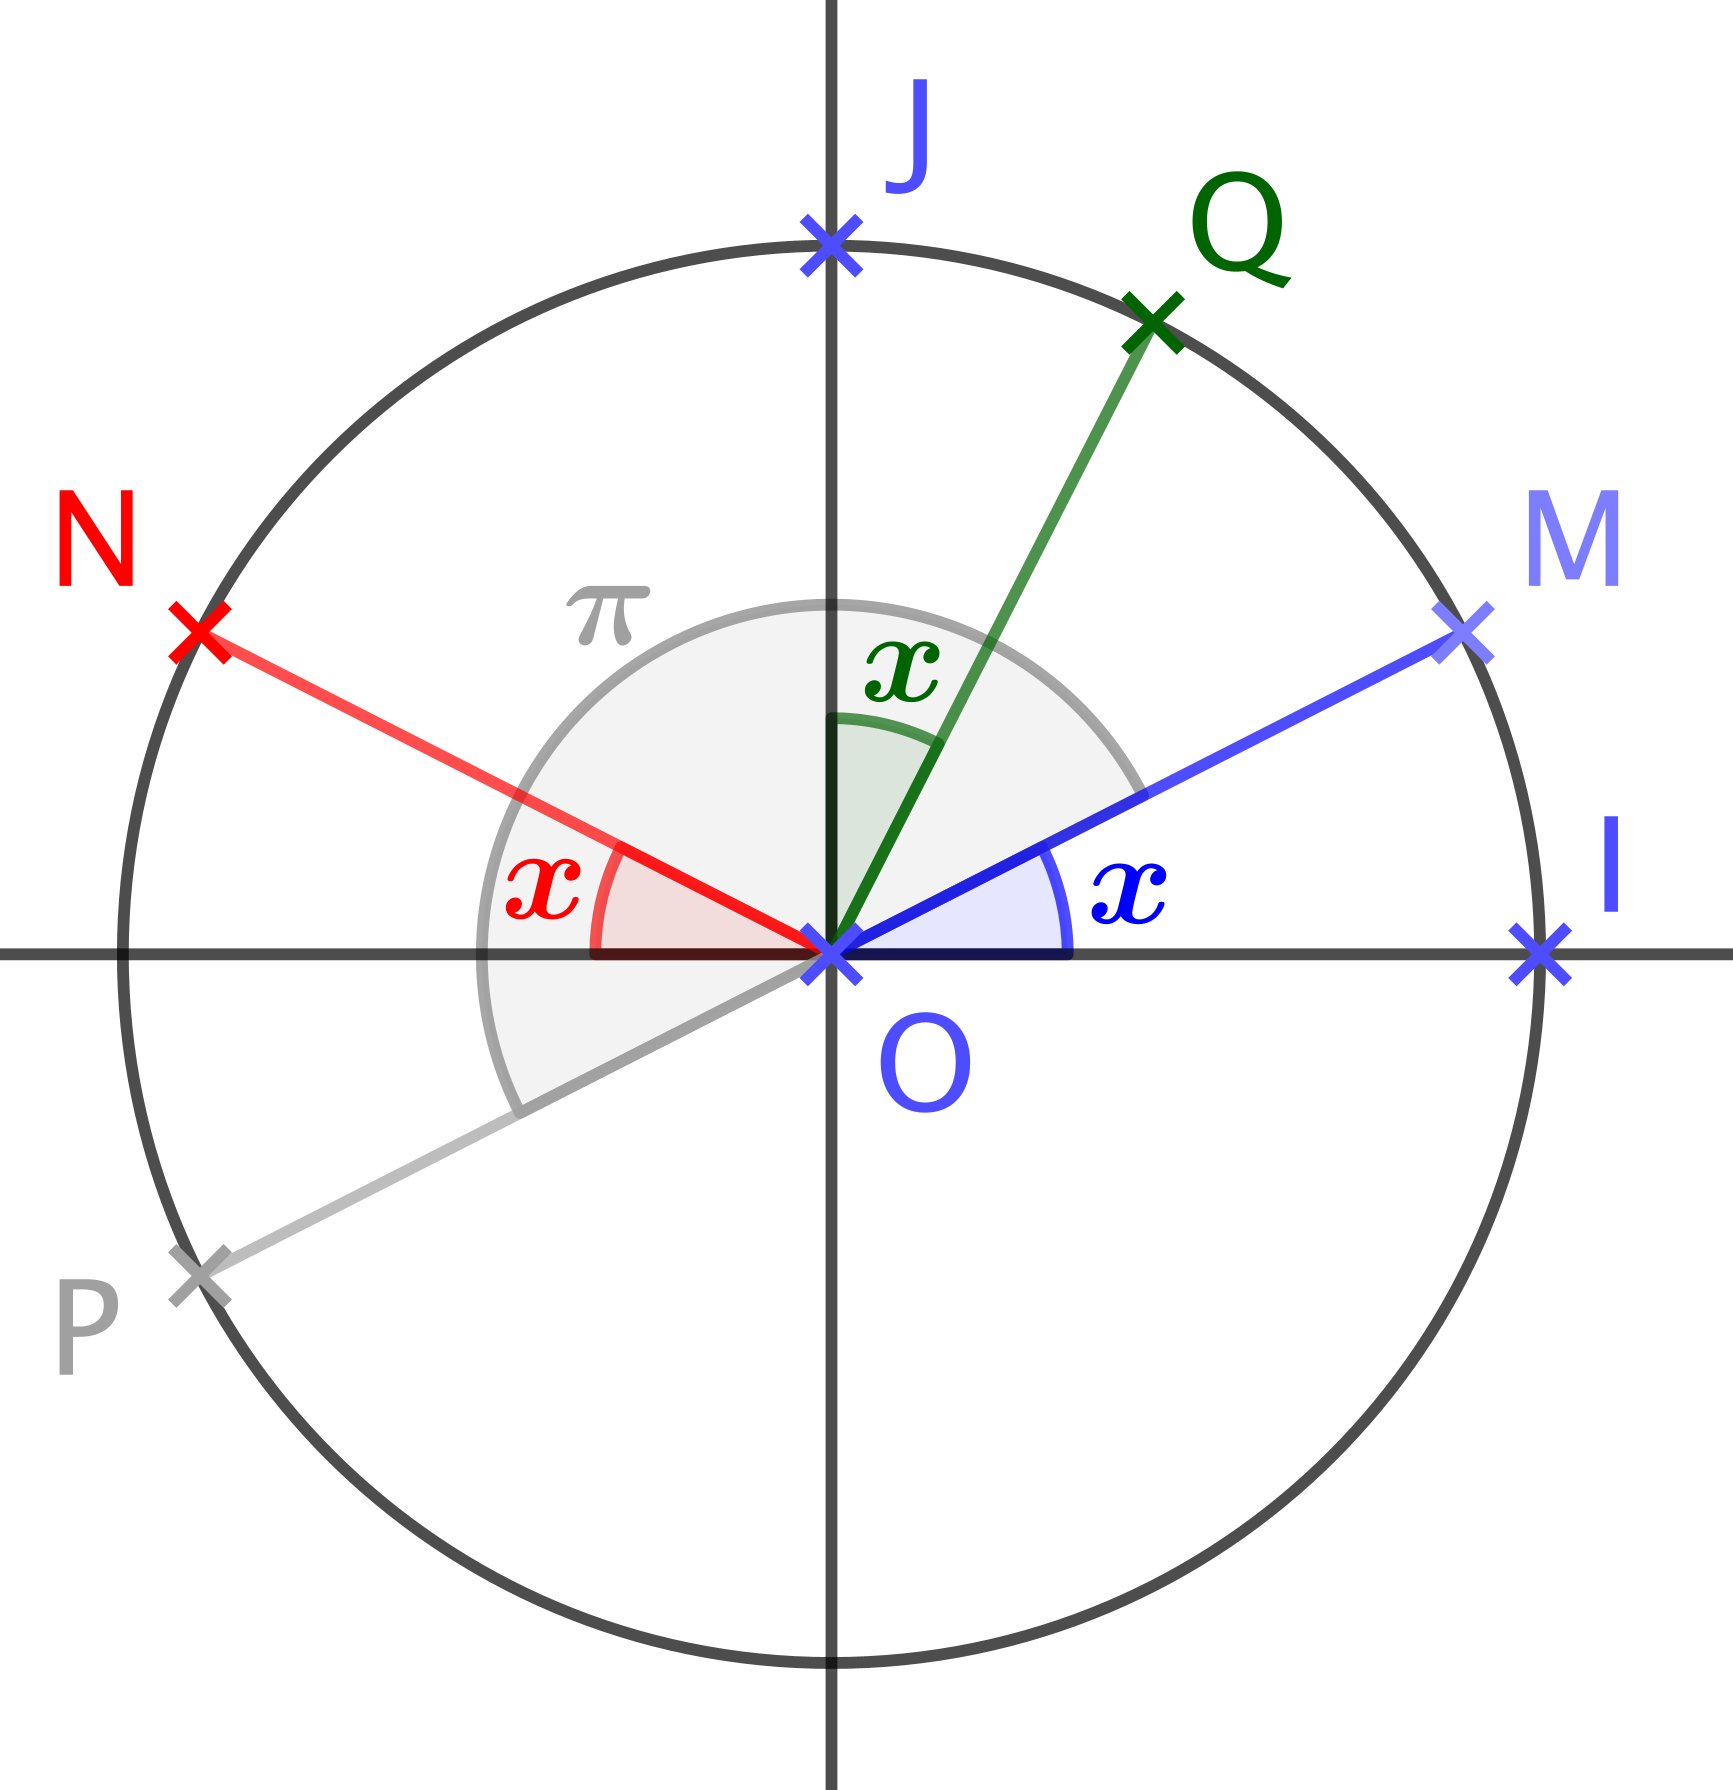
\includegraphics[scale = .7]{/trigo-identities/one-var-trig-formulas.png}}
\end{center}

Via les points $M$, $N$ , $P$ et $Q$, il est facile de fournir des arguments géométriques justifiant que, sous la condition $x \in \intervalO{0}{\frac{\pi}{4}}$, on a:
%
\begin{multicols}{3}
\begin{itemize}[label=\small\textbullet]
	\item $\cos (\pi - x) = - \cos x$

	      \noindent
	      $\sin (\pi - x) = \sin x$ 

	\item $\cos (x + \pi) = - \cos x$

	      \noindent
	      $\sin (x + \pi) = - \sin x$

	\item $\cos \left( \frac{\pi}{2} - x \right) = \sin x$

	      \noindent
	      $\sin \left( \frac{\pi}{2} - x \right) = \cos x$ 
\end{itemize}
\end{multicols}


De nouveau, il serait bien de pouvoir passer à la validité des formules précédentes sur $\RR$ tout entier sans plus d'effort \emph{(considérer les autres cas n'est pas compliqué, mais c'est pénible)}.
%
Nous allons voir que cela est licite grâce au fait \ref{holo-nullity} suivant qui est un peu technique, car il nécessite la notion de fonction holomorphe, un concept dont nous redonnons la définition tout de suite.


\begin{definition*}
    Soit $\Omega$ un ouvert non vide de $\CC$.
	Une fonction complexe $f: \Omega \rightarrow \CC$ est dite holomorphe en $\omega \in \Omega$, 
	si la limite 
	$\displaystyle \lim_{\stackrel{\abs{z - \omega} \, \rightarrow \, 0}{z \, \in \, \Omega - \setgene{\omega}}} \frac{f(z) - f(\omega)}{z - \omega}$
	existe dans $\CC$.
\end{definition*}


\medskip

Tout comme avec les fonctions réelles dérivables sur $\RR$, la propriété d'holomorphie se conserve par addition, multiplication, inverse et composition.
De plus, comme les fonctions polynomiales, les fonctions holomorphes vérifient des restrictions fortes sur leurs zéros éventuels, comme le montre le fait classique suivant.

\begin{fact} \label{holo-nullity}
    Soit $f: \Omega \rightarrow \CC$ une fonction non identiquement nulle, et holomorphe sur $\Omega$ un ouvert non vide de $\CC$.
    %
	Si $\lambda \in \Omega$ vérifie $f(\lambda) = 0$,
	alors il existe un ouvert $V$ tel que 
	$\lambda \in V \subseteq \Omega$,
	et
	$\forall z \in V - \setgene{\lambda}$, $f(z) \neq 0$ 
	\emph{(c'est le principe des zéros isolés d'une fonction holomorphe à une variable)}. 
\end{fact}


\begin{proof}
	Ceci nous amènerait trop loin, donc nous admettrons ce résultat.
\end{proof}


Si nous revenons à nos identités trigonométriques, il suffit de savoir que les fonctions circulaires réelles ne sont en fait que les restrictions à $\RR$ de fonctions holomorphes sur $\CC$ tout entier, et de noter que le raisonnement géométrique au début de cette section fait clairement apparaître des zéros non isolés pour les fonctions holomorphes sur $\CC$ suivantes.%
\footnote{
	Nous admettrons ces affirmations qui ne sont pas violentes à démontrer une fois que l'on a les bases de la théorie des fonctions holomorphes.
}
%
\begin{itemize}[label=\small\textbullet]
	\item $A(z) = \cos (\pi - z) + \cos z$ 
	   et $B(z) =\sin (\pi - z) - \sin z$ 

	\smallskip
	\item $C(z) =\cos (z + \pi) + \cos z$ 
	   et $D(z) =\sin (z + \pi) + \sin z$

	\smallskip
	\item $E(z) =\cos \left( \frac{\pi}{2} - z \right) - \sin z$ 
	   et $F(z) =\sin \left( \frac{\pi}{2} - z \right) - \cos z$ 
\end{itemize}


Que faire si nous avons des formules trigonométriques impliquant deux variables? Par exemple, le dessin suivant, par simple application des définitions géométriques du cosinus et du sinus, donne à la fois
$\cos(\alpha + \beta) = \cos \alpha \cos \beta - \sin \alpha \sin \beta$
et
$\sin(\alpha + \beta) = \cos \alpha \sin \beta + \sin \alpha \cos \beta$
pour
$(\alpha ; \beta) \in \big( \RRsp \big)^2$ tel que $0 < \alpha + \beta < \frac{\pi}{2}$. 

\begin{center}
	\fbox{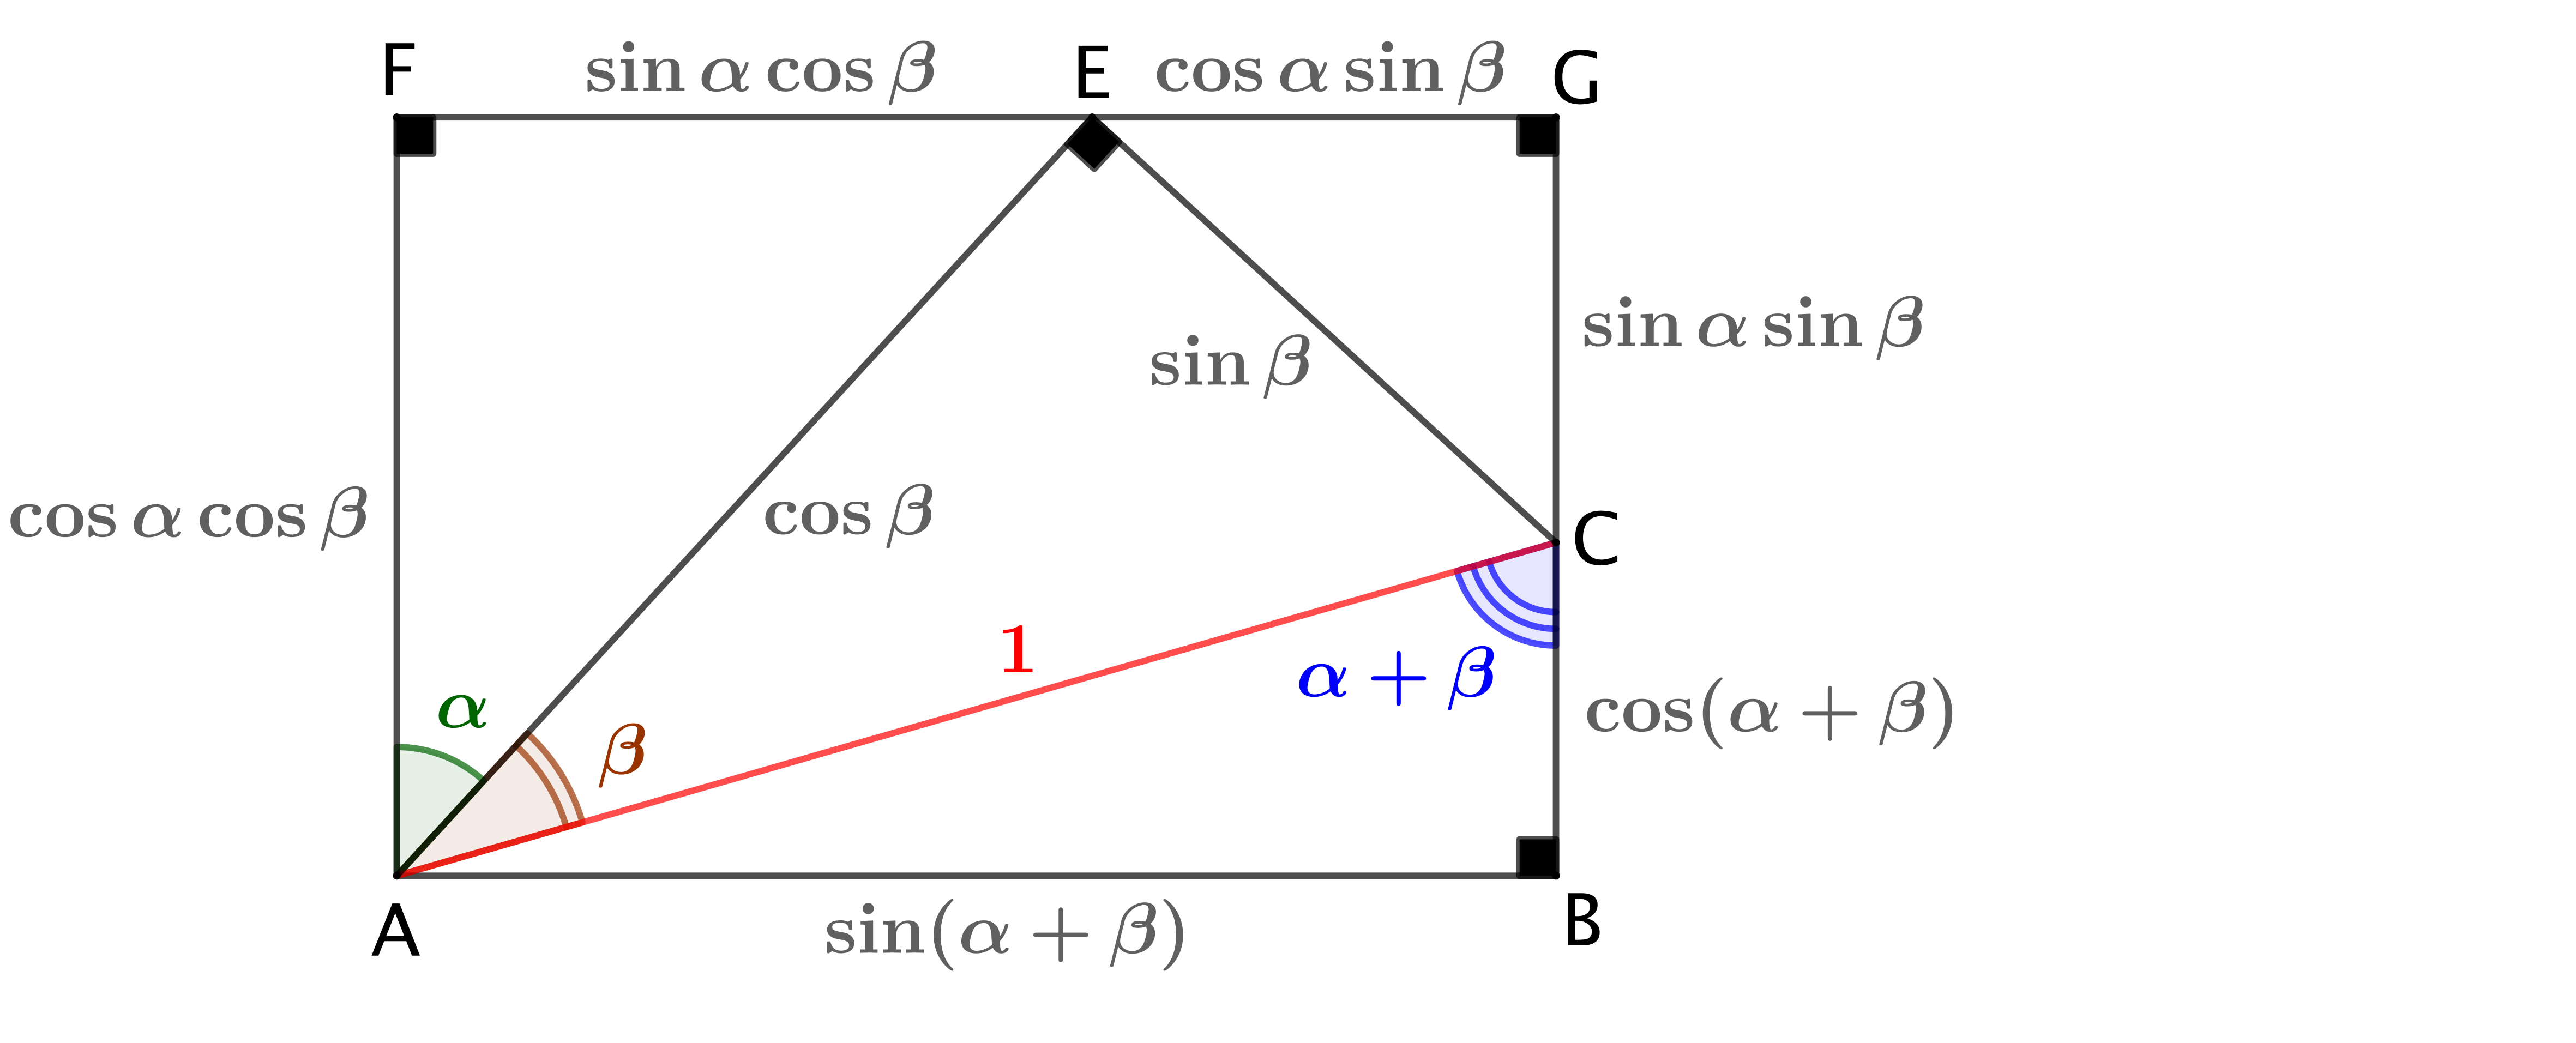
\includegraphics[scale = .7]{/trigo-identities/two-var-trig-formulas.png}}
\end{center}

La rigidité des fonctions holomorphes de plusieurs variables, voir le fait \ref{multi-holo-nullity} ci-dessous, implique la validité des formules trigonométriques précédentes sur $\RR^2$ tout entier.%
\footnote{
	Il suffit de considérer les fonctions holomorphes
	$(\alpha ; \beta) \in \CC^2 \mapsto \cos(\alpha + \beta) - \cos \alpha \cos \beta + \sin \alpha \sin \beta \in \CC$
	et
	$(\alpha ; \beta) \in \CC^2 \mapsto \sin(\alpha + \beta) - \cos \alpha \sin \beta - \sin \alpha \cos \beta \in \CC$.
}
Nous voilà sauvés!


\begin{definition*}
    Soit $\Omega$ un ouvert non vide de $\CC^n$ avec $n \in \NNs$.
	Une fonction complexe $f: \Omega \rightarrow \CC$ est dite holomorphe en $\omega \in \Omega$, 
	si elle est $\CC$-différentiable en $\omega$,
	c'est-à-dire s'il existe une application $\CC$-linéaire $Df: \CC^n \rightarrow \CC$
	vérifiant
	$\displaystyle \lim_{\stackrel{\norm{z - \omega}_n \, \rightarrow \, 0}{z \, \in \, \Omega - \setgene{\omega}}} \frac{f(z) - f(\omega) - Df(\omega) (z - \omega)}{z - \omega} = 0$.
\end{definition*}


\begin{fact} \label{multi-holo-nullity}
    Soit $f: \Omega \rightarrow \CC$ une fonction non identiquement nulle, et holomorphe sur $\Omega$ un ouvert non vide de $\CC^n$ avec $n \in \NN_{\geq 2}$.
    %
	L'ensemble des zéros de $f$ est un sous-ensemble analytique de $\Omega$ de codimension au moins $1$, c'est-à-dire de dimension au plus $(n-1)$.
\end{fact}


\begin{proof}
	Ceci nous amènerait bien trop loin, donc nous admettrons ce résultat. Si vous avez une impression de déjà-lu, c'est normal.
\end{proof}
